\documentclass{beamer}
\usepackage{graphicx}
\usepackage{paralist}
\usepackage{outlines}

\title{DAM 110 - Week 14 - How Digital Cameras Work, and Correcting Lens Flare \& Glare}
\author{Mendocino College - Digital Image Manipulation with Photoshop}
\titlegraphic{\vspace{-10mm}
\includegraphics[width = .9\textwidth]{images/photoshop.jpg}} 
\date{\vspace{-5em}} 


\mode <presentation>
\usetheme{Warsaw}
\usecolortheme{default}

\setbeamerfont{footline}{size=\fontsize{5}{8}\selectfont}

\definecolor{darkred}{rgb}{20,0,0}
\definecolor{darkgreen}{RGB}{40,110,20}
\definecolor{darkpurple}{RGB}{30,0,30}
\definecolor{chardonnay}{RGB}{255, 255, 204}

\setbeamercolor*{palette primary}{fg=white, bg=darkgreen}


\begin{document}
	{
		\setbeamertemplate{footline}{} 
		\setbeamertemplate{headline}{} 
		\begin{frame}
			\vspace{-35pt}
			\maketitle
		\end{frame}
	}

	\section{}
			\subsection{Lecture Topics}		
	\begin{frame}
		\frametitle{Lecture Topics for the Week}
				\begin{outline}
					\1 How Digital Cameras Work
					\1 Correcting for Lens Flare
					\1 Fixing Glare in Glasses
				\end{outline}
		\end{frame}

	\section{How Digital Cameras Work}
			\subsection{How Human Eyes Work}		
				\begin{frame}
					\frametitle{How Human Eyes Work}
					\begin{outline}
						\1 Iris
						\1 Lens
						\1 Rods and Cones
					\end{outline}
				\begin{center}
					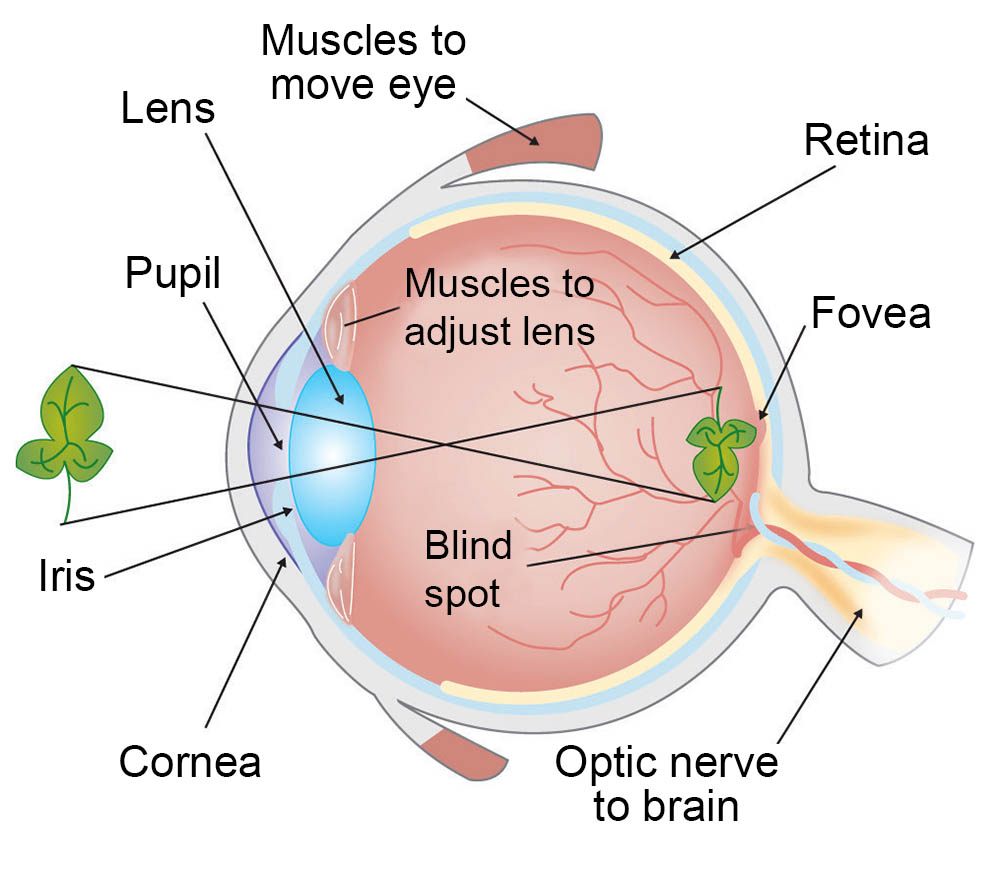
\includegraphics[width=0.65\textwidth]{images/eye-anatomy-1000.jpg}
				\end{center}
				\end{frame}

			\subsection{How Film Cameras Work}		
\begin{frame}
	\frametitle{How Film Cameras Work}
	\begin{outline}
		\1 Lens
		\1 Aperture
		\1 Film ISO speed
	\end{outline}
	\begin{center}
		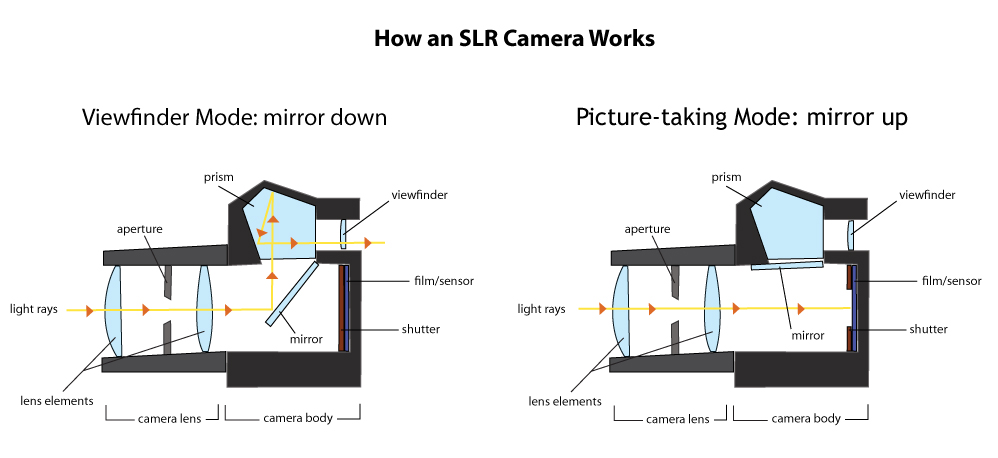
\includegraphics[width=1.0\textwidth]{images/How Camera Works.jpg}
	\end{center}
\end{frame}

			\subsection{How Digital Cameras Work}		
\begin{frame}
	\frametitle{How Digital Cameras Work}
	\begin{outline}
		\1 Sensors
		\1 Photosites
		\1 ISO Rating
	\end{outline}
	\begin{center}
		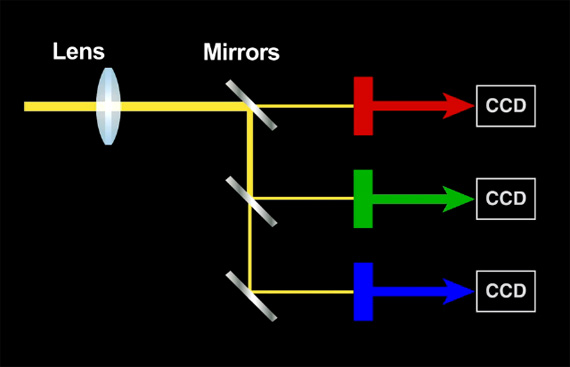
\includegraphics[width=1.0\textwidth]{images/digital-camera-work.jpg}
	\end{center}
\end{frame}
			
	\section{Lens Flare}
		\subsection{What is Lens Flare?}		
			\begin{frame}
				\frametitle{What is Lens Flare?}
				\begin{center}
				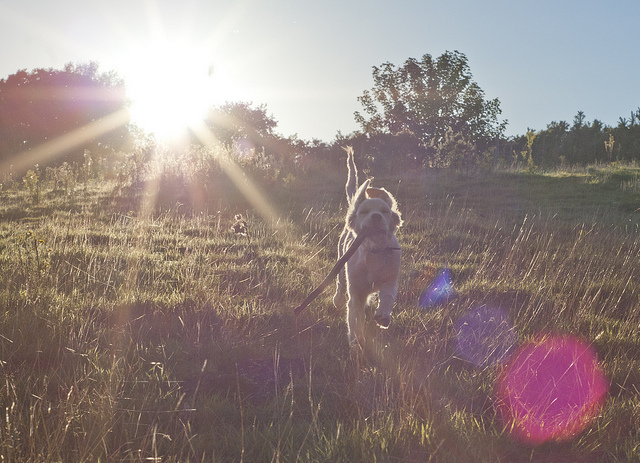
\includegraphics[width=1.0\textwidth]{images/Beautiful Lens Flare Photographs (13).jpg}
			\end{center}
			\end{frame}
		
		\subsection{How to Avoid Lens Flare}		
\begin{frame}
	\frametitle{How to Avoid Lens Flare}
	\begin{center}
		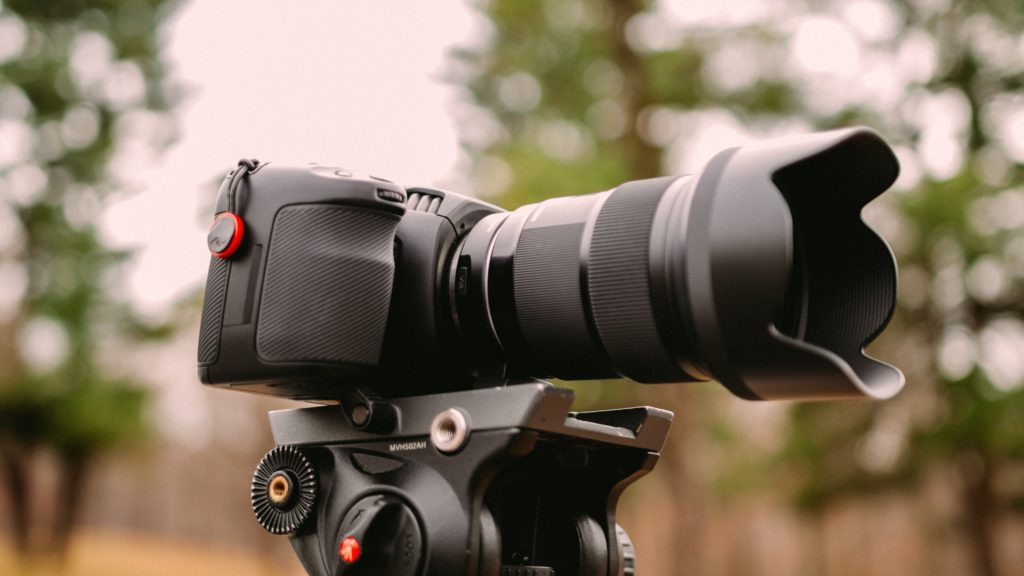
\includegraphics[width=1.0\textwidth]{images/kushagra-kevat-S1Tnl450Rtg-unsplash-1024x576-1.jpg}
	\end{center}
\end{frame}

		\subsection{Working with Lens Flare}		
\begin{frame}
	\frametitle{Using Lens Flare}
				\begin{center}
	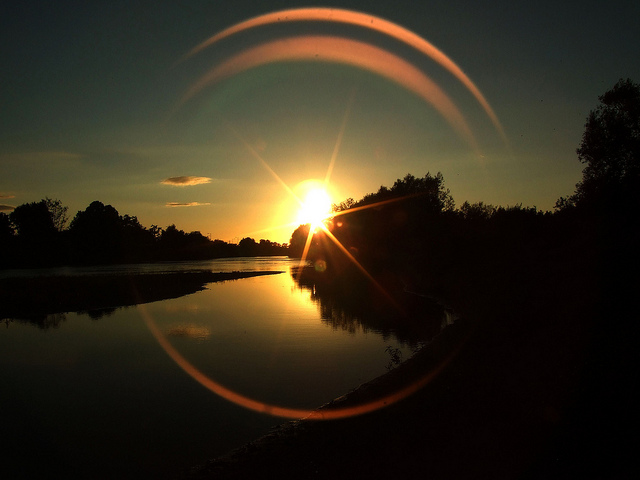
\includegraphics[width=1.0\textwidth]{images/Beautiful Lens Flare Photographs (11).jpg}
\end{center}
\end{frame}
		
\begin{frame}
	\frametitle{Adding Lens Flare}
	\begin{center}
		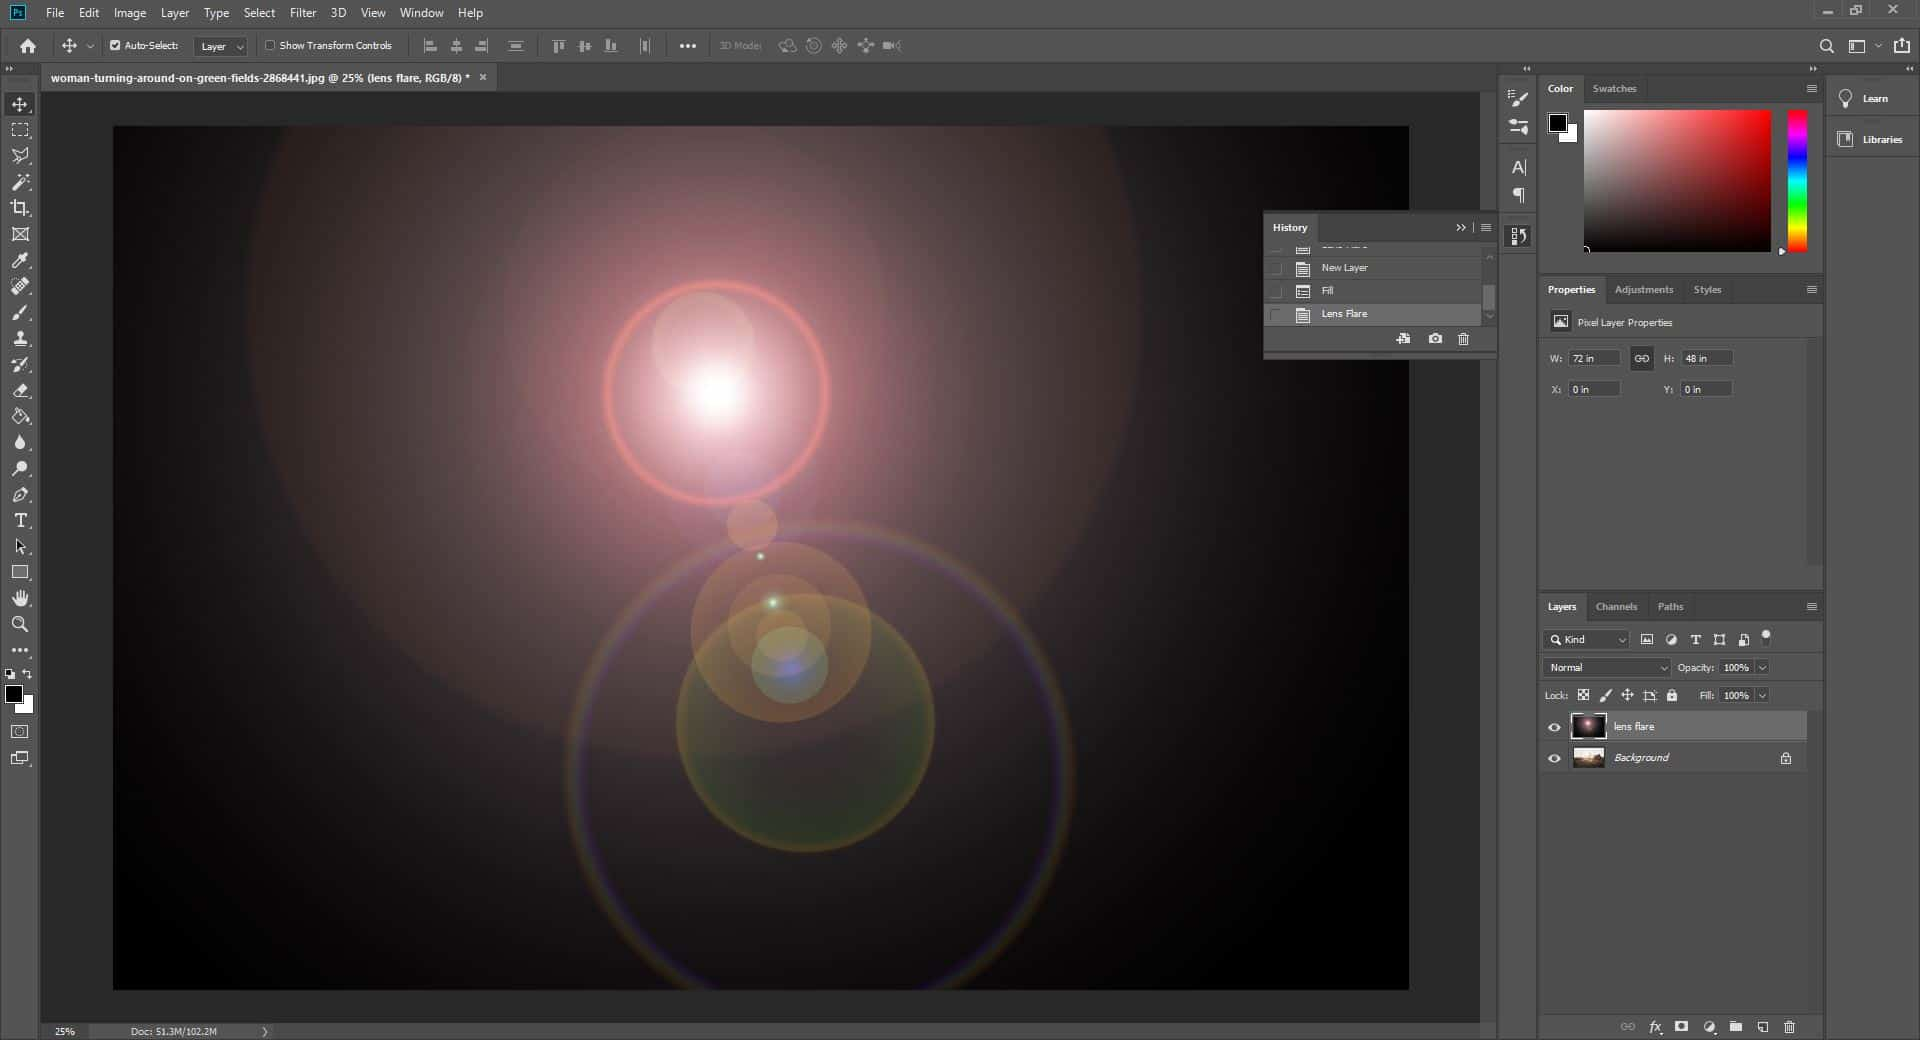
\includegraphics[width=1.0\textwidth]{images/lens-flare-14.jpg}
	\end{center}
\end{frame}
			
	\section{Glass Glare}
			\subsection{What is Glass Glare?}		
				\begin{frame}
					\frametitle{What is Glass Glare?}
					\begin{center}
					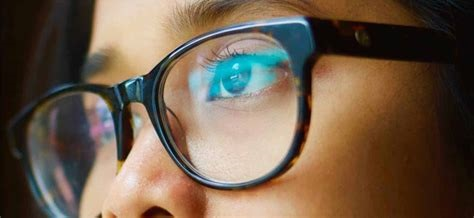
\includegraphics[width=1.0\textwidth]{images/glass glare.jpg}
				\end{center}
				\end{frame}

			\subsection{How to fix Glass Glare}		
\begin{frame}
	\frametitle{How to fix Glass Glare}
					\begin{center}
	
\includegraphics[width=1.0\textwidth]{images/remove glass glare.jpg}
\end{center}
\end{frame}

\section{Weekly Practice}

\subsection{Weekly Exercises}		
\begin{frame}
	\frametitle{Exercises for the Week}
	\begin{outline}
		\1 Practice Exercises this week:  
		\2 Fixing Lens Flare
		\2 Adding Lens Flare
		\2 Removing Glass Glare
		\1 Make a contact sheet with all of the original photos, with your modified images.
		\1 Submit the Contact Sheet
	\end{outline}
\end{frame}

\subsection{Assignment}		
\begin{frame}
	\frametitle{ Assignment}
	\begin{outline}
		\1 Two Final Mini-Project Images
		\2 Explain the changes you made.
		\2 Add your logo and post them to your portfolio site.
		\2 Submit the URLs to your images
	\end{outline}
\end{frame}

\subsection{Discussion}		
\begin{frame}
	\frametitle{Articles/Videos}
	\begin{outline}
		\1 How Cameras Work
		\2  By:  Tom Harris
		\2  Pages:  17
		\2 https://electronics.howstuffworks.com/camera.htm
		\1 DIGITAL CAMERA SENSOR SIZES
		\2  By:  Cambridge in Colour
		\2  Pages:  9
		\2  https://www.cambridgeincolour.com/tutorials/digital-camera-sensor-size.htm
		\1 How do digital cameras work? | James May Q\&A | Head Squeeze
		\2  By:  BBC Earth Lab
		\2  Duration:  4 minutes 34 seconds
		\2 https://youtu.be/Ic0czeUJrGE
	\end{outline}
\end{frame}

\begin{frame}
	\frametitle{Research Topics}
	\begin{outline}
		\1 Iris (human eye)
		\1 Lens (human eye)
		\1 Cornea (human eye)
		\1 Pupil (human eye)
		\1 Fovea (human eye)
		\1 Retina (human eye)
		\1 Rods (human eye)
		\1 Cones (human eye)
		\1 Light
		\1 Lens (camera)
		\1 Film
		\1 SLR (Single Lens Refractor) Camera's
		\1 DSLR Camera's
		\1 Negative (film)
		\1 Negative (digital)
	\end{outline}
\end{frame}
	
			
\end{document}